\chapter{Bestimmung der Halbwertsbreite}
\section{Durchführung}
Nach erfolgreichem Abschluss der Kalibrierung wird die Halbwertsbreite (FWHM - Full Width at Half Maximum) der dominanten Peaks bestimmt. Dies umfasst zwei Linien aus dem $^{60}Co$-Spektrum, die 661-keV-Linie von $^{137}Cs$ sowie bestimmte, gut aufgelöste Linien aus dem $^{152}$Eu-Spektrum. Aus der Halbwertsbreite und der Peakenergie wird die Energieauflösung des Detektors berechnet und die Energieabhängigkeit der Auflösung untersucht.

Im vorherigen Abschnitt wurde gezeigt, dass die Breite der Peaks im Halbleiterdetektors wesentlich schmaler ist als die eines Szintillationsdetektors. Dieser Unterschied lässt sich durch die Bestimmung der Halbwertsbreite (FWHM) der Photopeaks, bezeichnet als $\Delta E$, charakterisieren. Hierzu werden die beiden Parameter $(E, FWHM)$ aus den Tabellen \ref{taba_2} und \ref{taba_3} gegeneinander aufgetragen.

Der für einen Halbleiterdetektor zu erwartende theoretische Zusammenhang (bei dem die intrinsische Halbwertsbreite $\Delta E_d$ mit der Photonenenergie zunimmt) wird durch folgende Gleichung \ref{eq_2} beschrieben:
\begin{equation}
\Delta E (E_\gamma) = \sqrt{\Delta E_d(E_\gamma)^2+\Delta E_e^2}.
\end{equation}
\label{eq_2}
Die Intrinsische Anteil der Halbwertsbreite ergibt den Zusammenhang welches in Gleichung \ref{eq_3} dargestellt ist:
\begin{equation}
    \Delta E_d (E_\gamma) = c\cdot\sqrt{E_\gamma}
\end{equation}
\label{eq_3}

Abbildung \ref{fig:halbw_1_2} zeigt die in Abhängigkeit von der Intensität berechneten FWHM-Werte für beide Detektoren sowie die entsprechenden, aus den Gleichungen \ref{eq_2} und \ref{eq_3} abgeleiteten Funktionen.
\begin{figure}[htbp]
    \centering
    \begin{subfigure}[t]{0.48\textwidth}
        \centering
        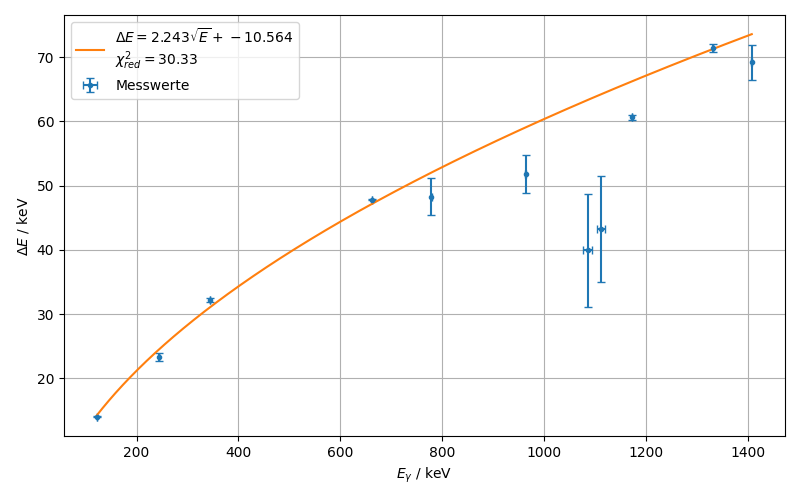
\includegraphics[width=\linewidth]{figs/Na(I)_Halbwertsbreite.png}
        \caption{NaI-Szintillationsdetektor}
        \label{fig:halbw_1_1}
    \end{subfigure}
    \hfill
    \begin{subfigure}[t]{0.48\textwidth}
        \centering
        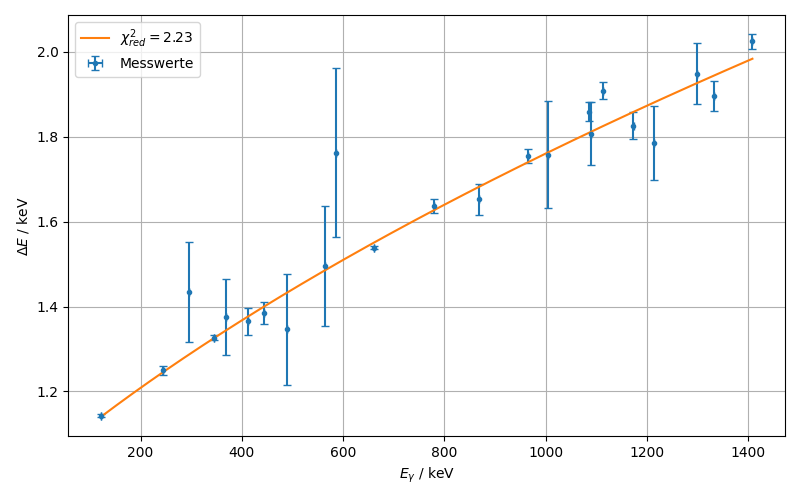
\includegraphics[width=\linewidth]{figs/Hablwertsbreite_richtig.png}
        \caption{HPGe-Halbleiterdetektor}
        \label{fig:halbw_1_2}
    \end{subfigure}
    \caption{FWHM-Halbwertsbreiten in Abhängigkeit von der Energie }
    \label{fig:halbw_1}
\end{figure}
% add plots

Der Vergleich der beiden Datensätze bestätigt, was bereits anhand der Intensitätsspektren zu beobachten war: Die dem Szintillationsdetektor zugeordnete Breite ist etwa 33-mal größer als die des Halbleiterdetektors.
% Beide Korrelationsfunktionen zeigen eine Breite der Photopeaks bei hohen reduzierten $\chi^2$-Wert (größer als 1). 
Lediglich beim NaI-Detektor tritt bei höheren Energien eine deutlichere Diskrepanz zwischen Modell und Messdaten auf.
Im Gegensatz dazu beträgt der reduzierte $\chi^2$-Wert des HPGe-Detektors lediglich $2.23$. Obwohl dieser Wert nicht exakt Eins entspricht, beschreibt das Modell die Messdaten insgesamt gut. Die zugrunde liegenden Messwerte sind in Tabelle \ref{tab:fwhm_messwerte} aufgeführt.

Die Fitparameter lauten wie folgt:

\begin{table}[H]
    \centering
    \caption{Fitparameter des Modells $\Delta E=\sqrt{\Delta E_\mathrm{e}^{\,2}+c^2E_\gamma}$ für den HPGe-Detektor.}
    \label{tab:fwhm_parameter}
    \begin{tabular}{lc}
        \toprule
        Parameter & Wert \\
        \midrule
        $\Delta E_\mathrm{e}$ / keV & $1.0249 \pm 0.0046$ \\
        $c$ / $\sqrt{\mathrm{keV}}$ & $0.04527 \pm 0.00024$ \\
        \bottomrule
    \end{tabular}
\end{table}

Im untersuchten Energiebereich liegt die Halbwertsbreite des HPGe-Detektors zwischen etwa $1.1\,\mathrm{keV}$ und $2.1\,\mathrm{keV}$. Der aus dem Fit bestimmte Wert $\Delta E_\mathrm{e}=(1.0249\pm0.0046)\,\mathrm{keV}$ beschreibt den energieunabhängigen elektronischen Beitrag zur Halbwertsbreite. Da dieser im gleichen Größenbereich wie die gemessene FWHM liegt, beeinflusst er insbesondere bei kleinen Energien die Energieauflösung deutlich. Mit zunehmender Photonenenergie dominiert dagegen der intrinsische, energieabhängige Beitrag des Detektors.
